\documentclass[letterpaper,12pt]{article}
\usepackage[utf8]{inputenc}
\usepackage[spanish]{babel}
\usepackage{float}
\usepackage{listings}
\usepackage{graphicx}
\usepackage{amsmath}
\usepackage{multicol}
\usepackage{fancyhdr}
\usepackage{caption}
\usepackage{parskip}
\usepackage[left=2.5cm,right=2.5cm,top=2.5cm,bottom=2.5cm]{geometry}

\pagestyle{fancy}
\fancyhf{}
\renewcommand{\headrulewidth}{0pt}
\renewcommand{\footrulewidth}{0pt}
\fancyhead[L]{
    \scriptsize
    Universidad de San Carlos de Guatemala\\
    Escuela de Ingeniería en Ciencias y Sistemas, Facultad de Ingeniería\\
    Introducción a la programación y computación 2, 1er. Semestre 2024
}
\fancyfoot[C]{\thepage}

\setlength{\headsep}{1.5cm}

\title{
    \rule{\textwidth}{0.4pt} \\
    \vspace{0.4cm}
    \textbf{SOLUCIÓN CON TIPOS DE DATOS ABSTRACTOS Y VISUALIZACIÓN DE DATOS} \\
    \rule{\textwidth}{0.4pt}
}
\author{202300476 – Alex Ricardo Castañeda Rodríguez}
\date{}

\begin{document}

\maketitle
\vspace{1cm}

\begin{multicols}{2}

    \section*{Resumen}
    El presente trabajo tiene como objetivo desarrollar una solución integral utilizando tipos de datos abstractos (TDA) y la visualización de datos mediante Graphviz, bajo el enfoque de la programación orientada a objetos (POO). Se busca implementar una lógica de manipulación de matrices basadas en archivos XML, optimizando la distribución de objetos de bases de datos en redes distribuidas. El proyecto aborda un problema NP-Hard mediante una metodología de agrupamiento para minimizar costos de transmisión y acceso.

    El enfoque propuesto no solo tiene como meta la minimización de costos, sino también la mejora de la eficiencia computacional mediante el uso de estructuras de datos abstractas, lo que permite un manejo eficiente de las tuplas y patrones de acceso.

    \textbf{Palabras clave:} Programación orientada a objetos, TDA, Graphviz, XML, NP-Hard.

    \section*{Abstract}
    This work aims to develop an integral solution using abstract data types (ADT) and data visualization through Graphviz, under the object-oriented programming (OOP) approach. It aims to implement matrix manipulation logic based on XML files, optimizing the distribution of database objects across distributed networks. The project addresses an NP-Hard problem through a clustering methodology to minimize transmission and access costs.

    The proposed approach not only seeks to minimize costs but also improves computational efficiency by using abstract data structures, allowing for efficient handling of tuples and access patterns.

    \textbf{Keywords:} Object-oriented programming, ADT, Graphviz, XML, NP-Hard.

    \newpage

    \section*{Introducción}
    La gestión y distribución de objetos de bases de datos en redes distribuidas es un problema crítico en sistemas modernos. Este proyecto se centra en optimizar la distribución de dichos objetos con el fin de reducir los costos de acceso y transmisión de datos. Los objetos de bases de datos pueden incluir atributos, relaciones, o archivos completos, y deben ser alojados en diferentes sitios de una red de forma que el acceso a estos sea eficiente.

    Este problema se complica aún más cuando se trata de grandes volúmenes de datos distribuidos, lo cual es característico de problemas NP-Hard. En este contexto, se propone una solución basada en la agrupación de tuplas con patrones de acceso similares, minimizando la redundancia y optimizando la transmisión de datos a lo largo de la red distribuida.

    La programación orientada a objetos (POO) proporciona un marco robusto para implementar este tipo de soluciones, permitiendo una mejor organización del código, mayor reutilización de componentes y una más clara separación de responsabilidades. Además, se utiliza la herramienta Graphviz para visualizar gráficamente las matrices de frecuencia de acceso y sus respectivas versiones reducidas.

    \begin{figure}[H]
        \centering
        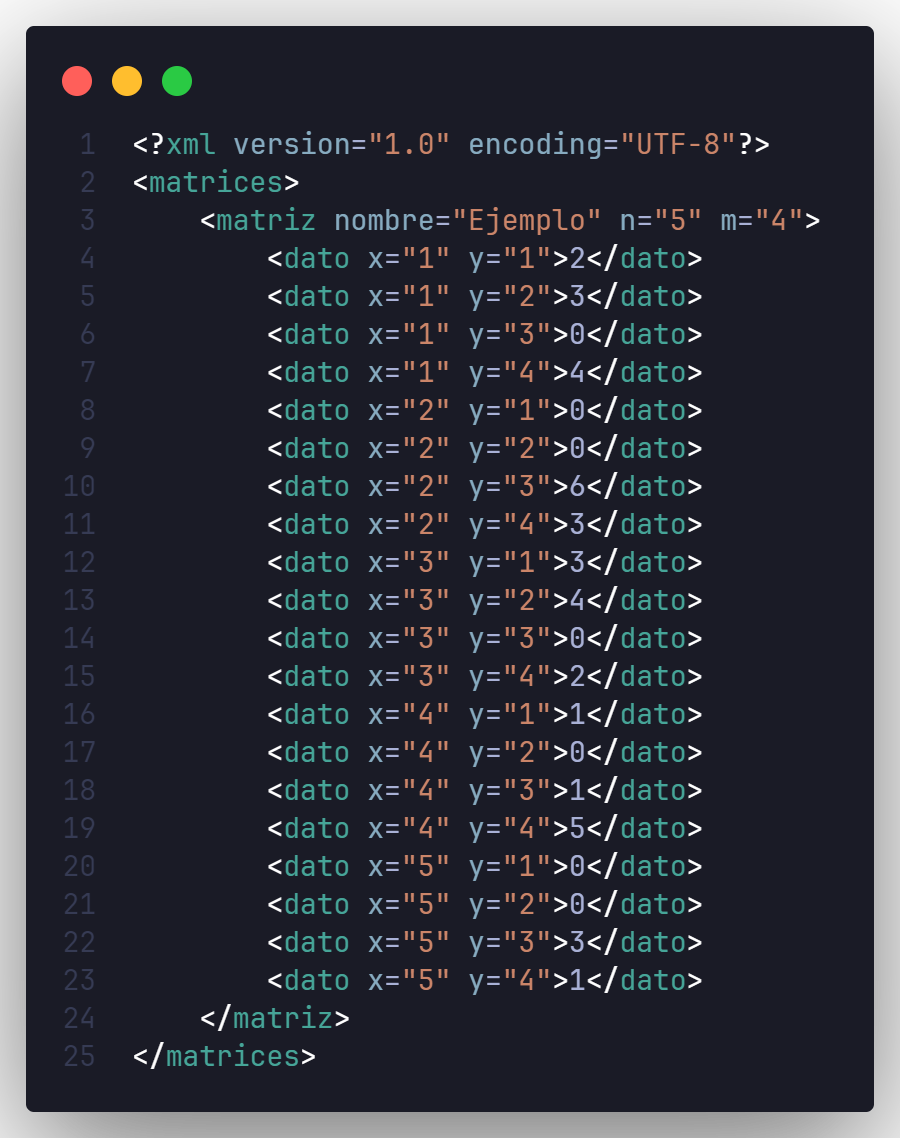
\includegraphics[width=\columnwidth]{images/xml_structure.png}
        \caption{Ejemplo de la estructura del archivo XML de entrada.}
    \end{figure}

    \section*{Objetivos}
    \textbf{Objetivo General:}
    Desarrollar una solución integral que implemente tipos de datos abstractos (TDA) y visualización de datos (Graphviz) bajo el concepto de programación orientada a objetos (POO).

    \textbf{Objetivos Específicos:}
    \begin{itemize}
        \item Implementar POO para el desarrollo de la solución a través de lenguaje Python.
        \item Utilizar estructuras de programación secuenciales, cíclicas y condicionales.
        \item Visualizar TDA's por medio de la herramienta Graphviz.
        \item Utilizar archivos XML como insumos para la lógica y comportamiento de la solución.
        \item Desarrollar una metodología de agrupamiento que permita optimizar la distribución de tuplas.
    \end{itemize}

    \section*{Desarrollo del tema}
    El proyecto aborda el problema de distribución de objetos de bases de datos en redes distribuidas, que debe ser resuelto de manera eficiente para minimizar los costos de transmisión y acceso. La solución se basa en la manipulación de matrices de frecuencia de acceso, que describen cuántas veces cada tupla es accedida desde cada sitio.

    La primera parte del proyecto consiste en la lectura de matrices de frecuencia desde archivos XML. Estos archivos están organizados en etiquetas como `<matrices>`, `<matriz>` y `<dato>`, y contienen toda la información necesaria para procesar las matrices. Una vez leídas, las matrices se analizan para identificar patrones de acceso similares entre las tuplas.

    \subsection*{Método de agrupamiento}
    Para optimizar la distribución de objetos en la red, se utiliza un método de agrupamiento que identifica patrones de acceso idénticos entre las tuplas. El objetivo es agrupar estas tuplas en conjuntos, lo que reduce la cantidad de datos transmitidos entre los sitios. Este proceso de agrupamiento genera una nueva matriz reducida, que contiene la suma de las frecuencias de acceso de las tuplas que pertenecen a un mismo grupo.

    \subsection*{Estructuras y algoritmos implementados}
    El diseño del programa se basa en una estructura de nodos y listas circulares simplemente enlazadas. Cada nodo representa una matriz, y las operaciones como la búsqueda de matrices duplicadas o la agrupación de tuplas se realizan mediante el recorrido de estas listas. Este enfoque permite una organización eficiente de los datos y facilita la validación de la existencia de matrices duplicadas.

    \begin{figure}[H]
        \centering
        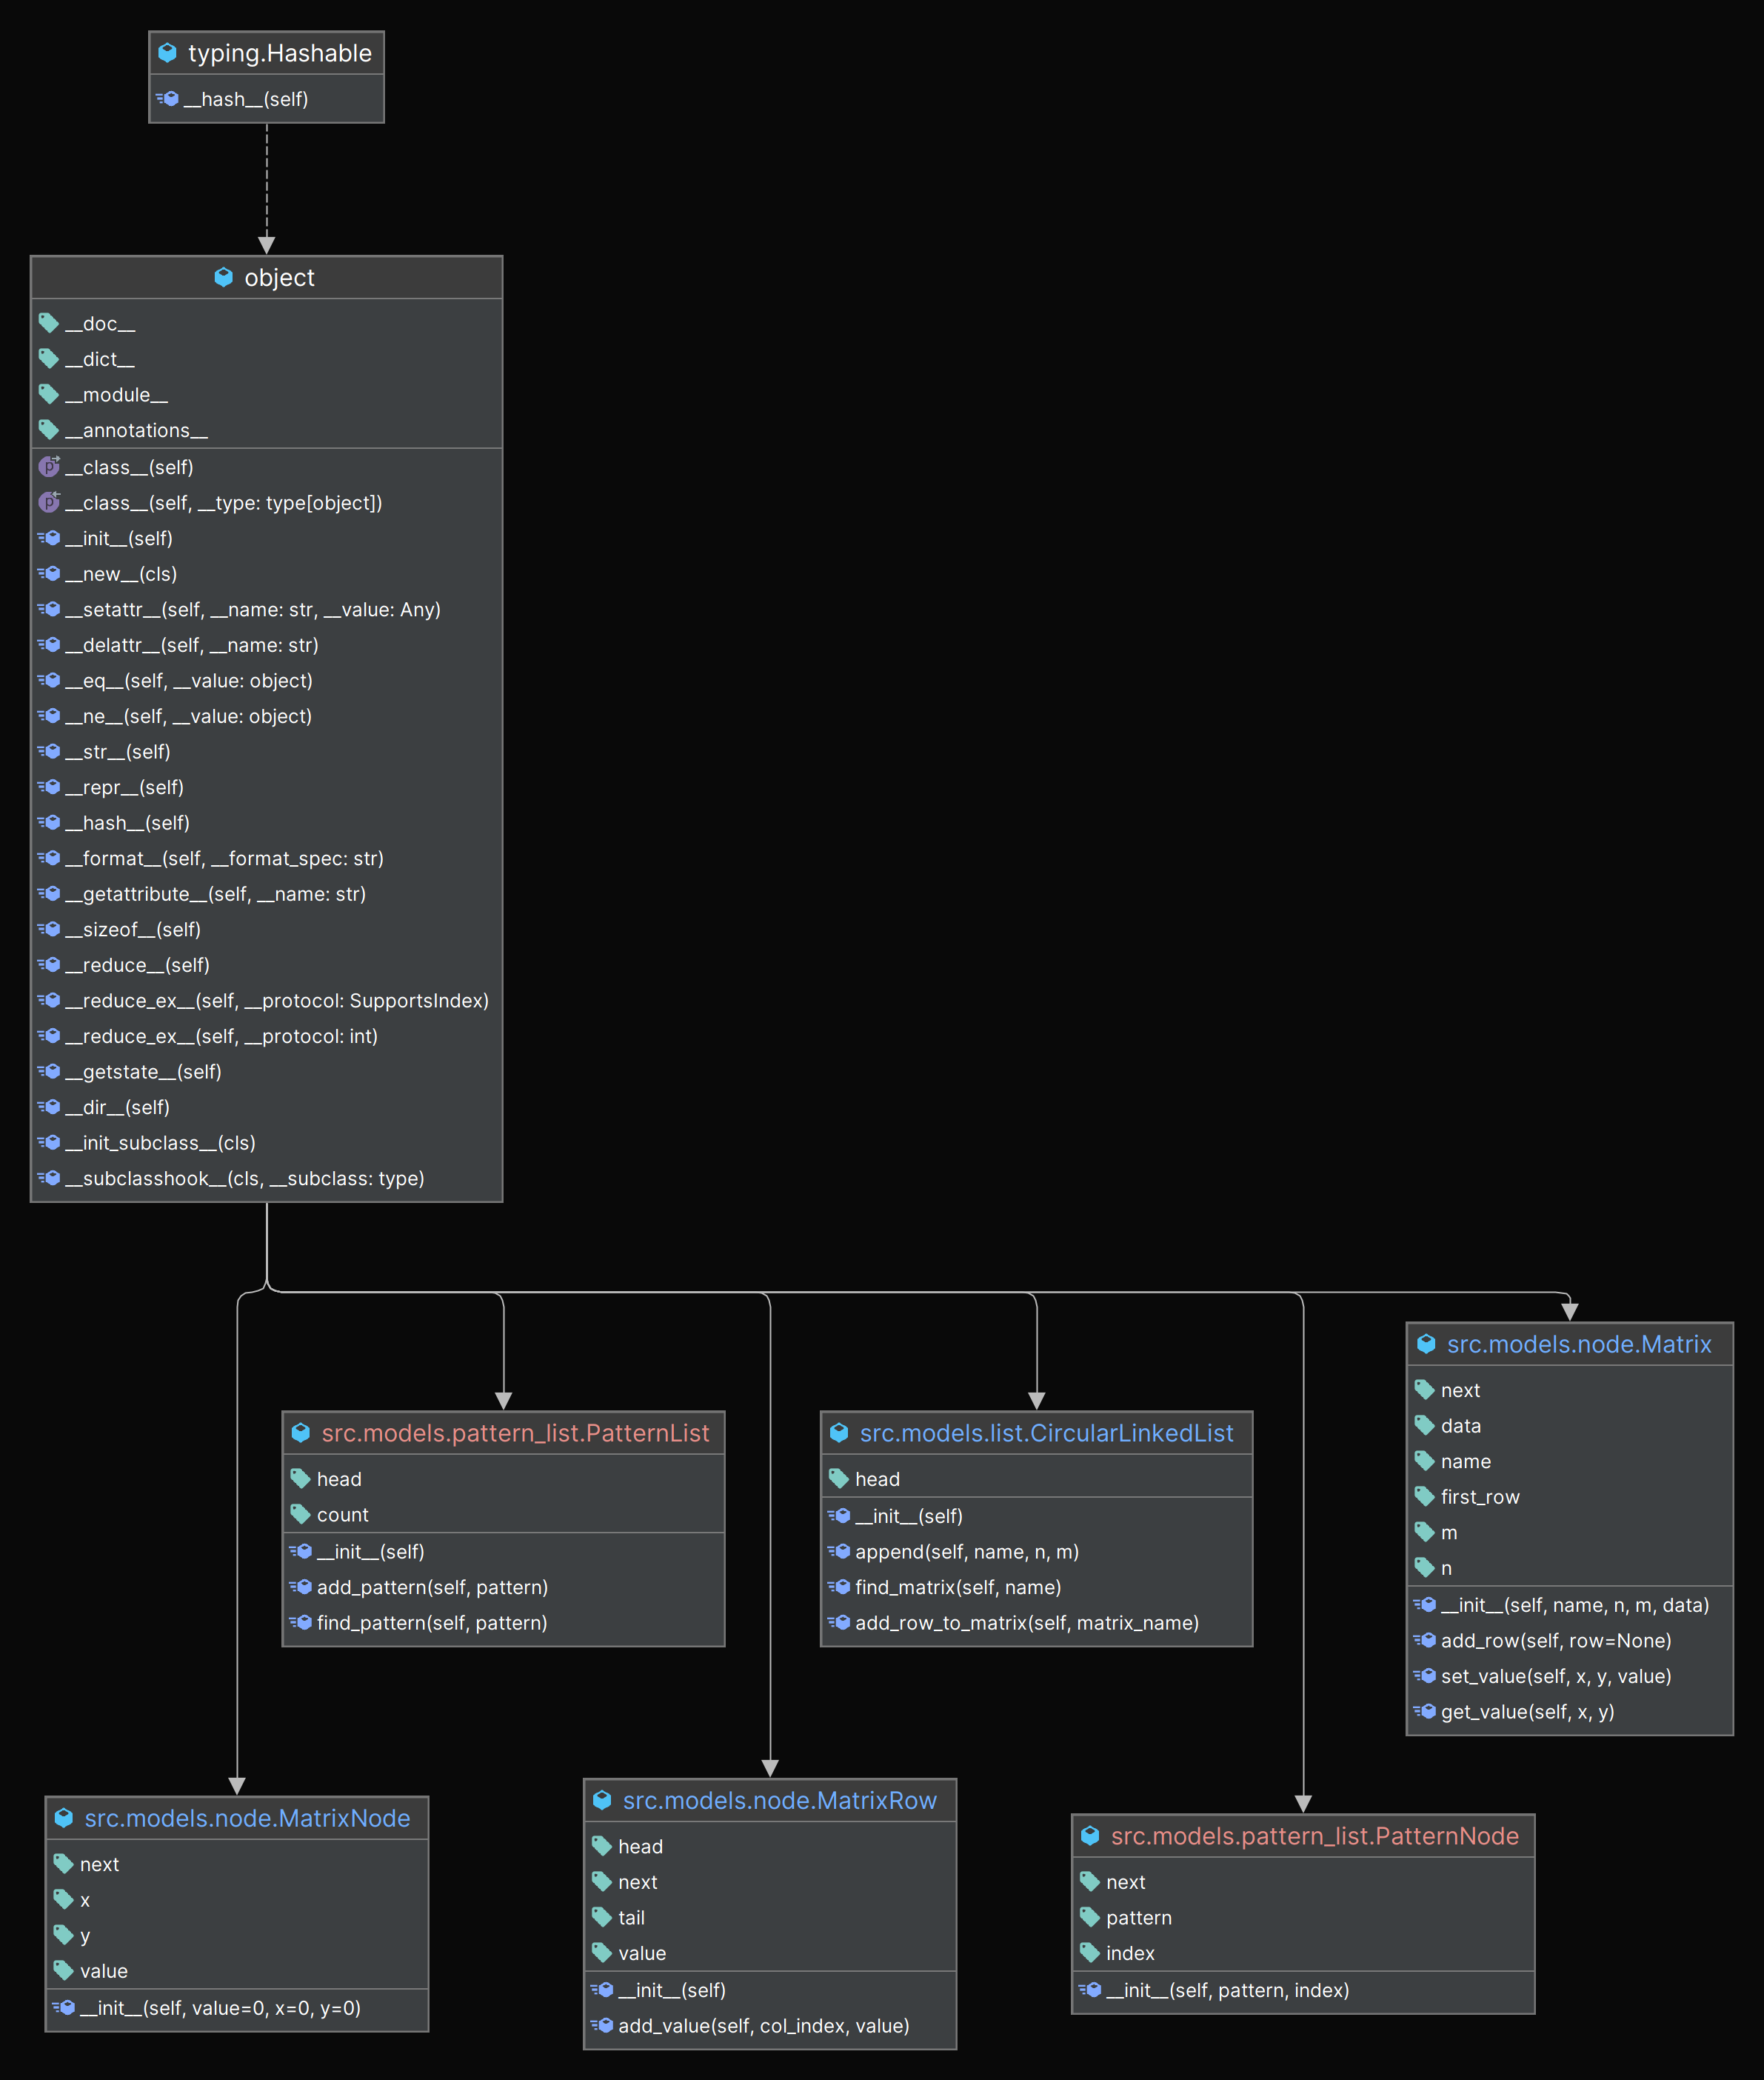
\includegraphics[width=\columnwidth]{images/class_diagram.png}
        \caption{Diagrama de clases que modela la solución orientada a objetos.}
    \end{figure}

    \newpage

    \section*{Ejecución del programa}
    El sistema se ejecuta mediante un menú de consola que proporciona varias opciones al usuario:

    \begin{enumerate}
        \item \textbf{Cargar archivo:} Permite cargar el archivo XML que contiene las matrices de frecuencia de acceso. El sistema valida que el archivo esté correctamente estructurado y muestra mensajes informativos sobre el estado de la carga.
        \item \textbf{Procesar el archivo:} Procesa la información cargada y agrupa las tuplas que comparten patrones de acceso. Durante este proceso, se muestra información en consola sobre los grupos que se están formando.
        \item \textbf{Escribir archivo de salida:} Genera un archivo XML con la matriz de frecuencia reducida. Este archivo contiene las mismas etiquetas que el archivo de entrada, pero las frecuencias han sido agrupadas en función de los patrones de acceso.
        \item \textbf{Mostrar datos del estudiante:} Muestra los datos del estudiante encargado del proyecto, como el nombre, carné, curso, y carrera.
        \item \textbf{Generar gráfica:} Utiliza Graphviz para generar dos gráficos: uno que muestra la estructura de la matriz original y otro que muestra la matriz reducida. Estos gráficos se generan en formato .dot y pueden visualizarse con la herramienta Graphviz.
        \item \textbf{Salir:} Finaliza la ejecución del programa.
    \end{enumerate}

    \begin{figure}[H]
        \centering
        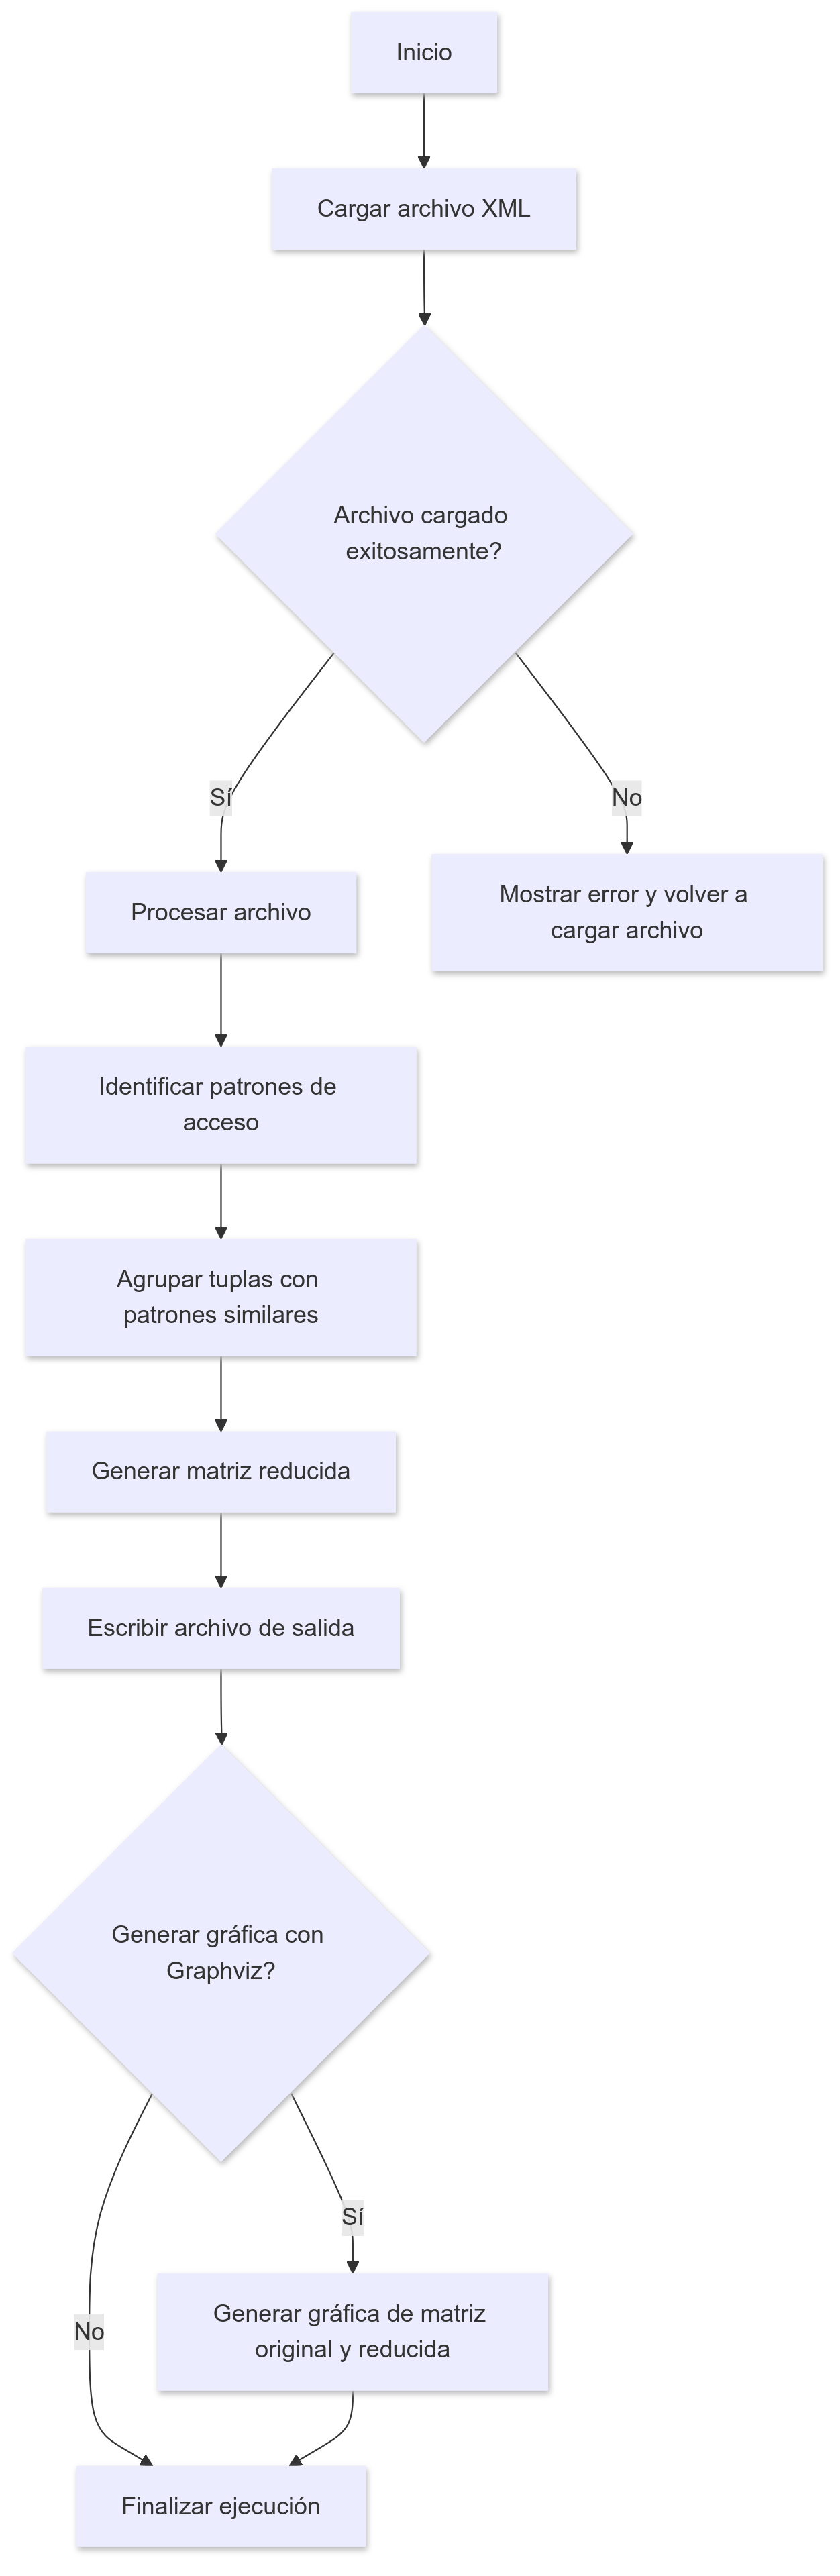
\includegraphics[width=\columnwidth]{images/activity_diagram.png}
        \caption{Diagrama de actividades que muestra el flujo del programa desde la carga del archivo hasta la generación de la salida.}
    \end{figure}

    \section*{Reportes y visualización}
    Para facilitar la comprensión de la solución propuesta, se incluye la generación de gráficos mediante la herramienta Graphviz. Estos gráficos muestran tanto la estructura de la matriz original como la de la matriz reducida, permitiendo observar cómo las tuplas se agrupan en función de sus patrones de acceso. Los gráficos incluyen detalles como el nombre de la matriz, el número de filas y columnas, y los valores contenidos en cada celda.

    \subsection*{Generación de gráficos}
    La generación de gráficos se basa en la lectura de la estructura del archivo XML y en la creación de nodos para cada una de las celdas de la matriz. A través de Graphviz, se genera un archivo .dot que puede ser renderizado en diversos formatos gráficos, como PNG o PDF.

    \begin{figure}[H]
        \centering
        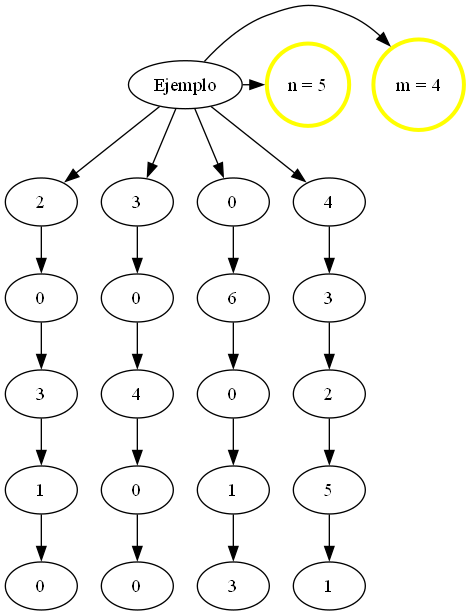
\includegraphics[width=\columnwidth]{images/matrix_graph_Ejemplo.png}
        \caption{Ejemplo de gráfico generado con Graphviz para una matriz de acceso.}
    \end{figure}

    \newpage

    \section*{Conclusiones}
    La solución presentada en este proyecto permite procesar matrices de acceso de manera eficiente, agrupando las tuplas con patrones de acceso similares para reducir los costos de transmisión en redes distribuidas. La implementación en Python bajo el paradigma de programación orientada a objetos facilita la reutilización de código y la modularidad del sistema. Adicionalmente, la visualización mediante Graphviz proporciona una herramienta útil para analizar el comportamiento de las matrices procesadas.

    La propuesta es escalable y puede adaptarse a diferentes escenarios donde la transmisión y acceso a bases de datos distribuidas sean factores clave. En futuros trabajos, se podría explorar la posibilidad de implementar algoritmos más avanzados para el agrupamiento de tuplas y la optimización de costos.

    \newpage
    \section*{Anexos}

    \subsection*{Anexo 1: Código Fuente en Python}
    A continuación se muestra un fragmento del código fuente implementado en Python para la lectura y procesamiento de archivos XML, así como la agrupación de matrices de acceso:

    \begin{figure}
        \centering
        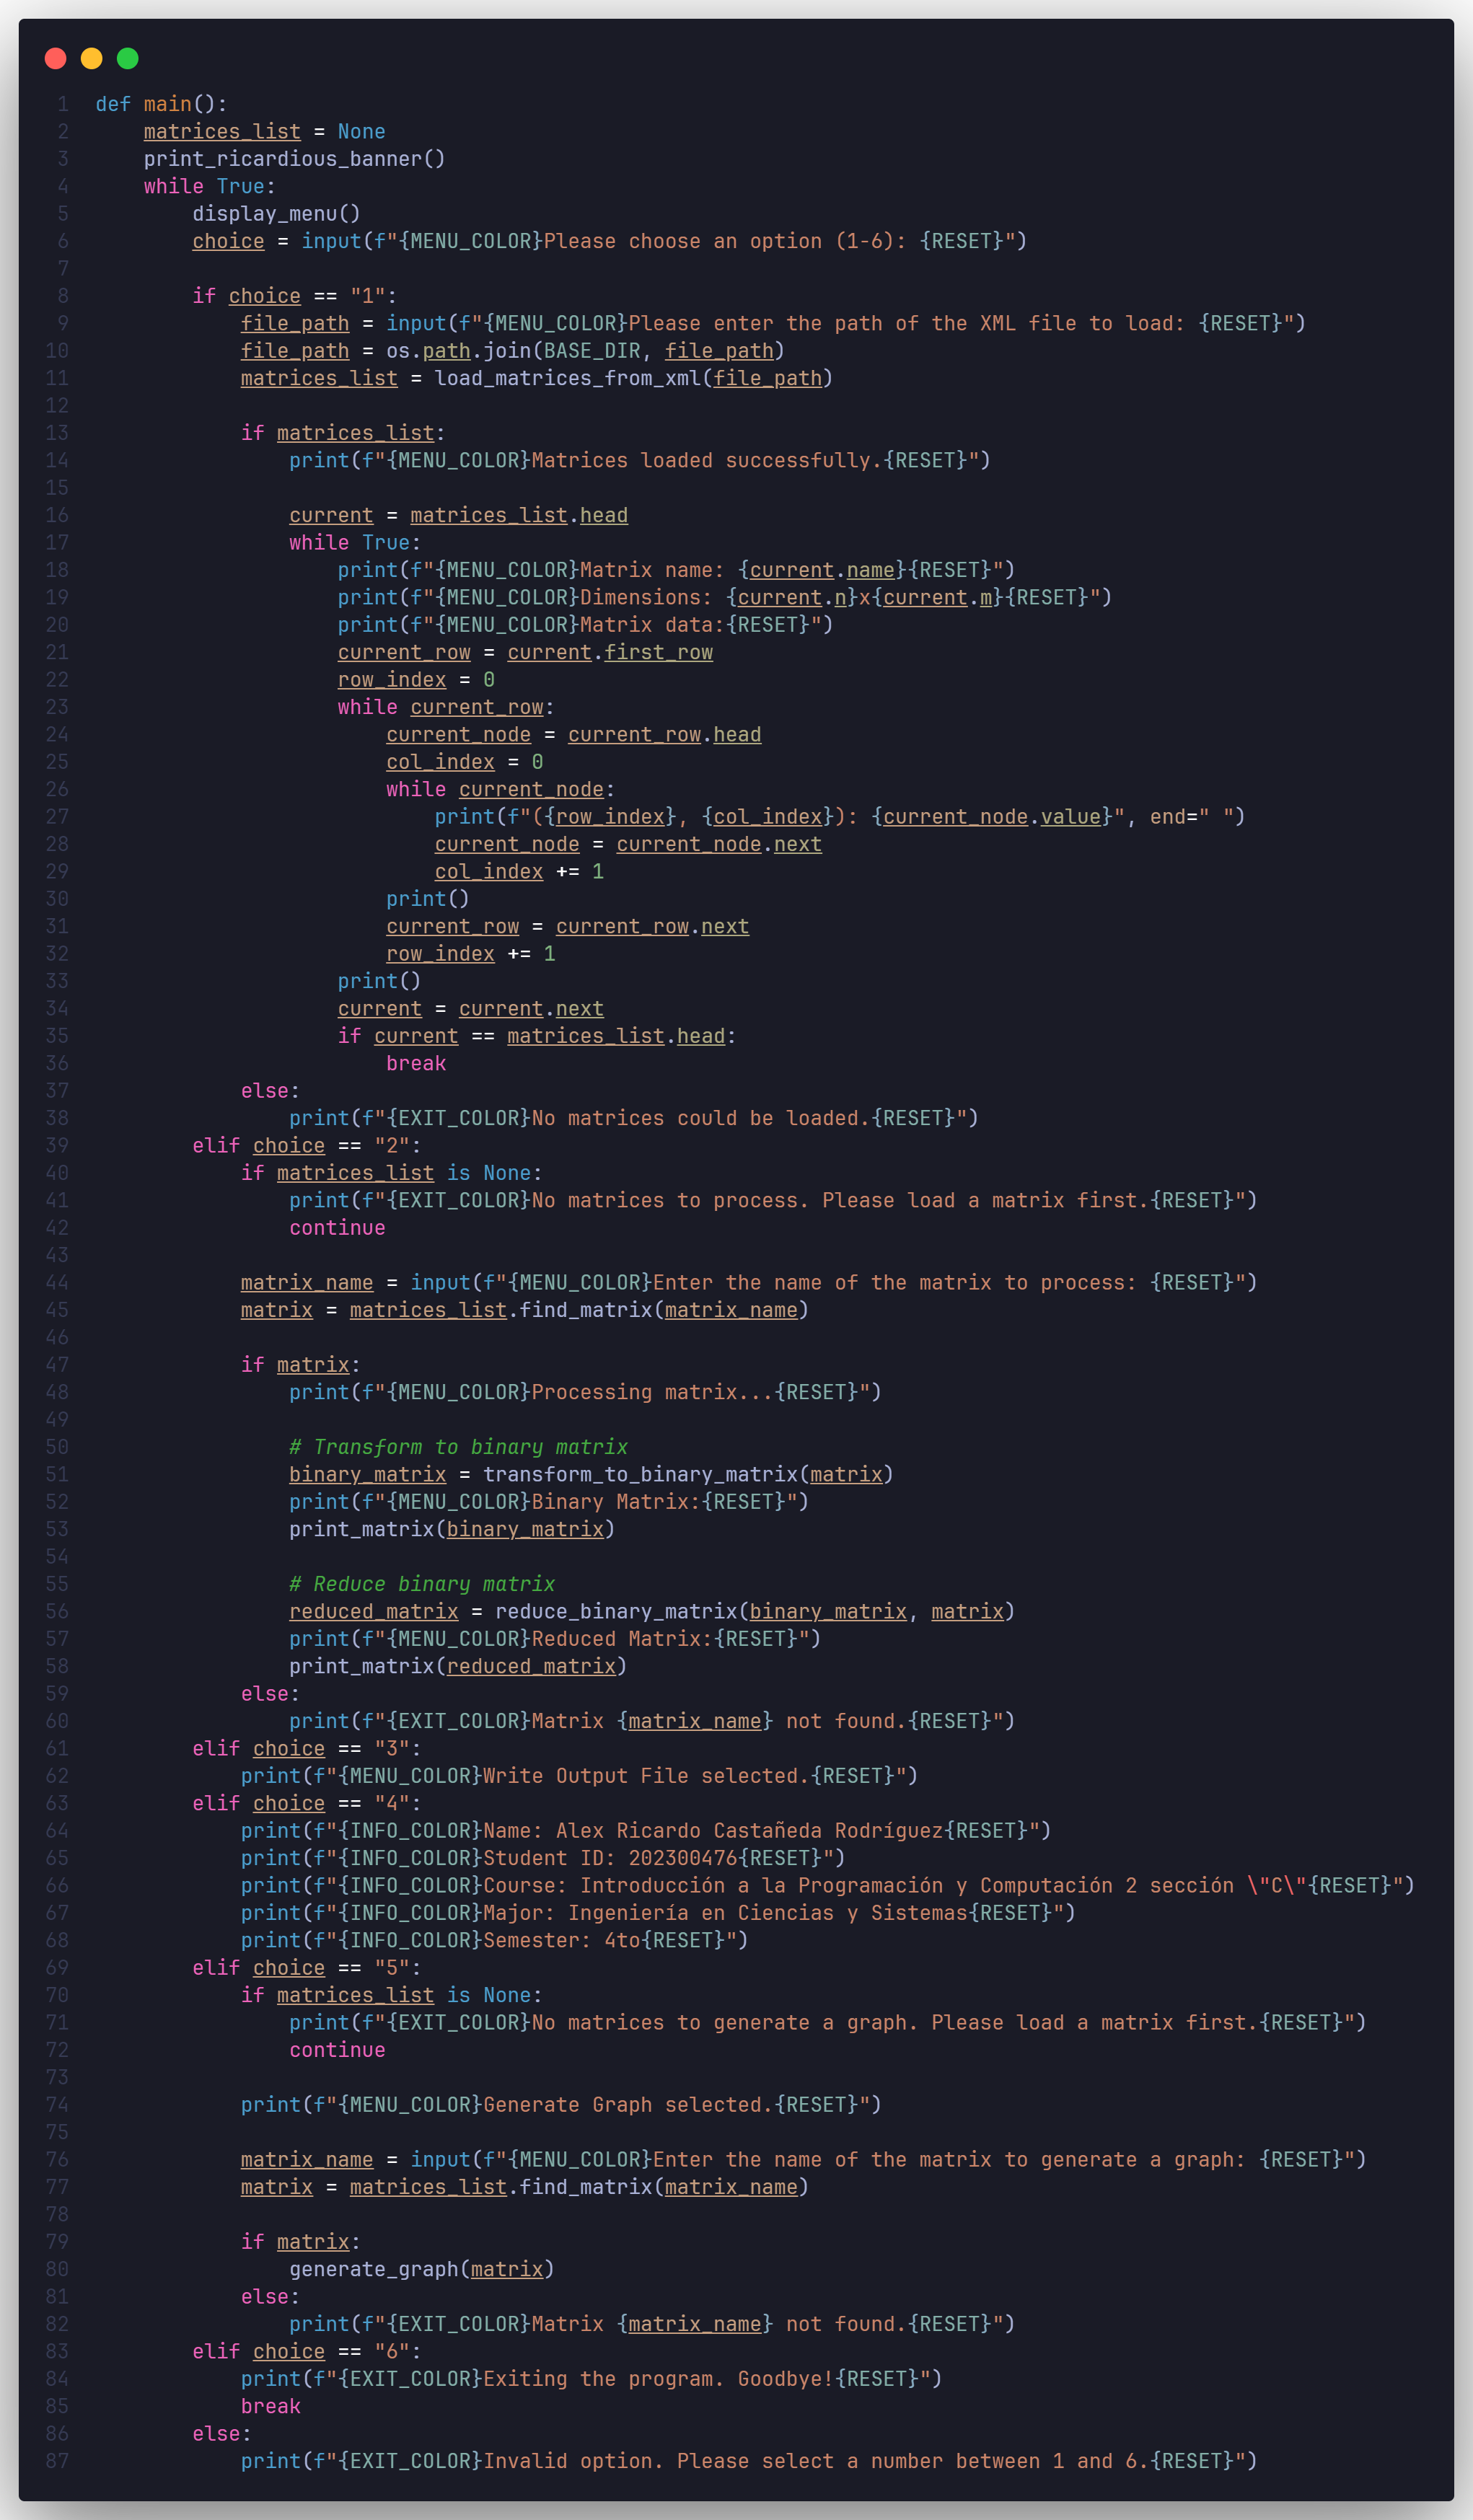
\includegraphics[width=\columnwidth]{images/screenshot_code.png}
        \caption{Fragmento de código fuente en Python para la lectura y procesamiento de matrices de acceso.}
    \end{figure}

    Este fragmento de código muestra cómo se leen las matrices desde el archivo XML y se procesan para identificar patrones de acceso.

    \subsection*{Anexo 2: Ejemplo de archivo XML de entrada}
    El siguiente es un ejemplo de un archivo XML que contiene la matriz de frecuencia de acceso. Este archivo sirve como insumo para el sistema desarrollado:

    \begin{figure}[H]
        \centering
        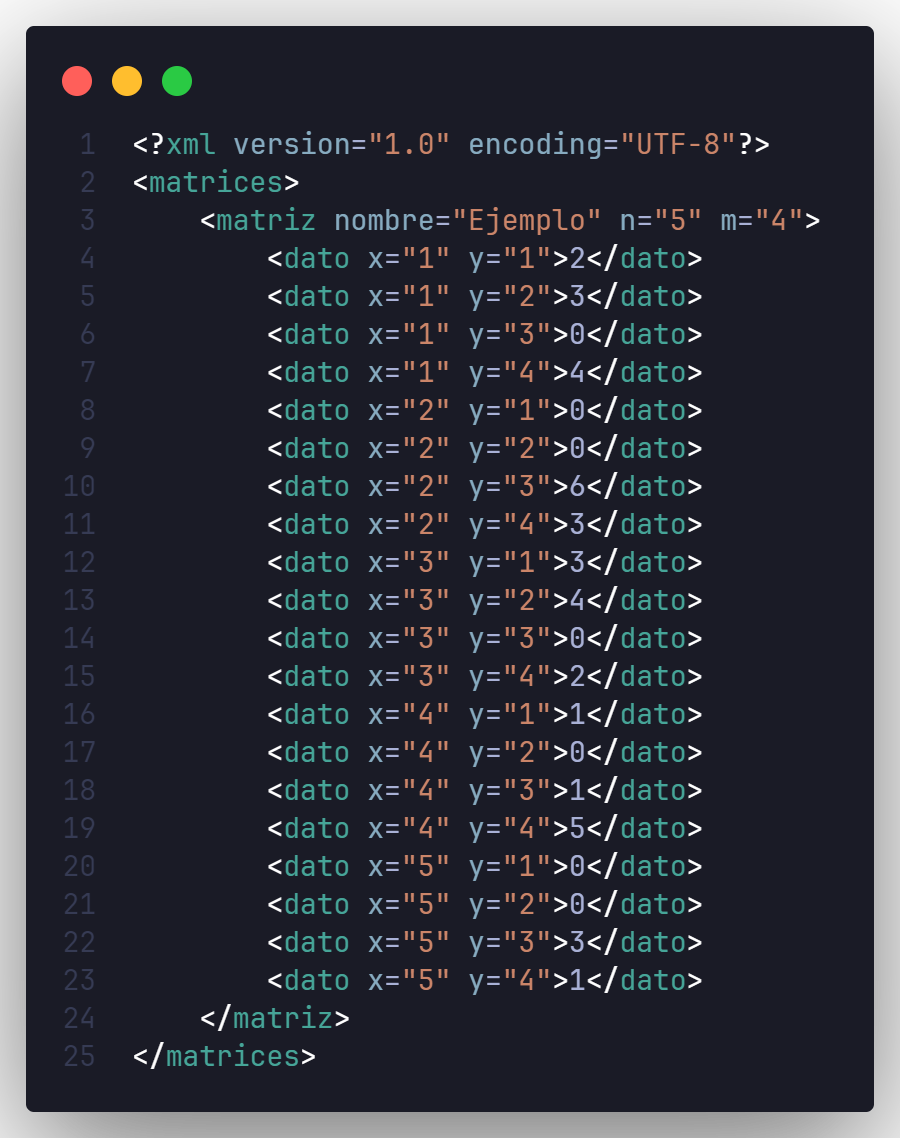
\includegraphics[width=\columnwidth]{images/xml_structure.png}
        \caption{Ejemplo de archivo XML que contiene la matriz de frecuencia de acceso.}
    \end{figure}

    Este archivo define una matriz de 4x4 donde cada dato está etiquetado con su posición `x` y `y`, y su valor correspondiente.


    \subsection*{Anexo 3: Manual de Usuario}
    El siguiente es un manual básico de usuario que describe cómo ejecutar y utilizar el sistema para procesar archivos XML y generar gráficos de matrices:

    \begin{itemize}
        \item \textbf{Paso 1:} Ejecute el programa desde la consola utilizando el comando `python main.py`.
        \item \textbf{Paso 2:} Seleccione la opción "Cargar archivo" en el menú de la consola e ingrese la ruta del archivo XML de entrada.
        \item \textbf{Paso 3:} Seleccione la opción "Procesar archivo" para agrupar las tuplas con patrones de acceso similares.
        \item \textbf{Paso 4:} Seleccione "Generar gráfica" para visualizar la matriz procesada mediante Graphviz.
        \item \textbf{Paso 5:} Opcionalmente, seleccione "Escribir archivo de salida" para generar un nuevo archivo XML con la matriz agrupada.
        \item \textbf{Paso 6:} Para finalizar, seleccione la opción "Salir" para cerrar el programa.
    \end{itemize}

    Este manual guía al usuario a través de las opciones disponibles en el sistema para cargar y procesar archivos, así como generar gráficos.

    \subsection*{Anexo 4: Capturas de Pantalla}
    A continuación se muestra una captura de pantalla del sistema en ejecución, donde se observa el menú principal y los mensajes informativos mostrados al usuario:

    \begin{figure}[H]
        \centering
        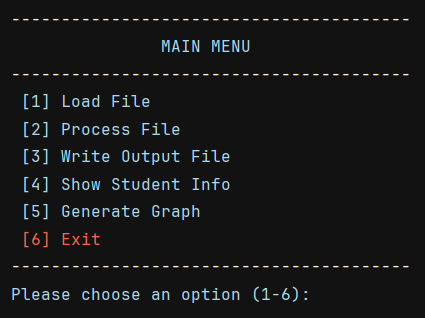
\includegraphics[width=\columnwidth]{images/screenshot_menu.png}
        \caption{Captura de pantalla del menú principal del sistema.}
    \end{figure}

    Esta imagen muestra cómo se visualiza el sistema de menús desde la consola.



    \section*{Referencias}
    \begin{itemize}
        \item Grady Booch, (1994). \textit{Object-Oriented Analysis and Design with Applications}. Benjamin/Cummings Publishing Company.
        \item Robert C. Martin, (2002). \textit{Agile Software Development, Principles, Patterns, and Practices}. Prentice Hall.
        \item E. Gamma, R. Helm, R. Johnson, J. Vlissides. \textit{Design Patterns: Elements of Reusable Object-Oriented Software}. Addison-Wesley.
    \end{itemize}

\end{multicols}

\end{document}
